Quando correntes balanceadas circulam pelos enrolamentos trifásicos do estator, um campo magnético senoidal distribuído gira no entreferro da máquina. O efeito produzido por este campo é similar ao produzido por um par de polos girando no entreferro, de tal forma que a distribuição de densidade de fluxo ao longo deste entreferro seja senoidal com o pico ao longo do eixo dos polos magnéticos.

\begin{figure}[ht!]
\center 
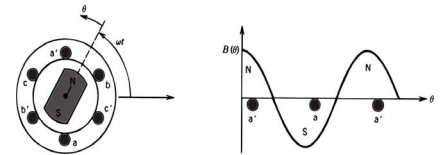
\includegraphics[scale=1.2]{imagens/14.PNG}
\caption{Distribuição de densidade de fluxo ao longo do entreferro.}\label{fig:14}
\end{figure}

A densidade do fluxo ao longo do entreferro é representado por:

$$B(\theta) = B_{max}. \cos(\theta)$$

A força eletromotriz, que é dada pela variação do fluxo no tempo multiplicada pelo número de espiras, permite escrever a expressão.

$$e_a = \omega . N. {\phi}_p . K_w = E_{max} . \sin(\omega t)$$

A tensão eficaz por fase:

$$E_1 = 4,44 . f_1 . N_1 . \phi_p . K_w$$

Com o fator de enrolamento $K_w$ variando de 0,85 à 0,95.

